% !TeX root = ../pyfracpaq-user-manual-en.tex
\major{Prepare the environment and start the application}\label{sec:inicio}
Obtain the code folder from GitHub by cloning the repository or downloading its ZIP. Open the folder containing \code{run_gui.py} and \code{requirements.txt}. Normal use requires Python 3.13 and the libraries; installing the PyFracPaQ package itself is unnecessary.

\subsection{Python and a virtual environment}
On macOS, with Python 3.13 available, run these commands from the project root:
\begin{verbatim}
python3.13 -m venv .venv
.venv/bin/python -m pip install -r requirements.txt
.venv/bin/python -m pip check
.venv/bin/python run_gui.py
\end{verbatim}
Alternatively, use \code{.venv/bin/python -m pyfracpaq} from the same folder. Obtaining the libraries may initially require internet access; subsequent analyses run locally. Do not silently change the versions pinned in requirements.txt.

\subsection{Miniforge and VS Code}
With Miniforge, prepare a separate environment:
\begin{verbatim}
conda create -n pyfracpaq python=3.13 pip
conda activate pyfracpaq
python -m pip install -r requirements.txt
python -m pip check
python run_gui.py
\end{verbatim}
In VS Code, open the folder and use \control{Python: Select Interpreter}. Select the Python executable in \code{.venv} or your Miniforge environment. Run \code{run_gui.py} or one of the supplied Run and Debug configurations. The Python extension supports selection and execution; Python Debugger is required for the debugging configurations.

CPython 3.13.18 and Miniforge/Python 3.13.13 have been checked on macOS arm64. Windows/Linux remain subject to future testing by the maintainer, rather than certified platforms. An environment already named pyfracpaq may use another version: check \code{python --version} before installing the libraries.

\subsection{What the folder needs to contain}
The application uses \code{pyfracpaq/}, its resources, the launcher and the libraries. \code{examples/} and this manual support normal use. Tests, audit reports and internal scripts are development material in the full clone and are not required at run time. The usage ZIP excludes them. The MATLAB distribution is not required.

\subsection{Working directory and existing files}
The usual output destination is the current working directory. Starting from the project root writes results there. To keep analyses separate, use a working copy or start the absolute path to \code{run_gui.py} from the output folder, using the prepared Python executable. Without installing the project, module execution should start at the project root.

Reusing a tag reuses and replaces the same filenames. Some intermediate files have fixed names without a tag. Preserve original inputs and separate analyses before clicking Run. SVG conversion is an exception to the output location: its TXT files are written beside the SVG.

\major{Inputs, geometry, scaling and orientation}\label{sec:dados}
\subsection{Traces, segments and nodes}
A \emph{trace} is the polyline representing a mapped fracture. Its vertices are input nodes; consecutive nodes define a segment. These geometric nodes are not automatically the topological I/Y/X nodes calculated later.

For \(\mathbf p_i=(x_i,y_i)\),
\begin{equation}
\ell_i=\|\mathbf p_{i+1}-\mathbf p_i\|_2,
\qquad L=\sum_i\ell_i.
\end{equation}
Total length \(L\) follows the path, rather than the straight distance between the endpoints. A trace centre is interpolated halfway along that path. A segment centre is the mean of its endpoints. These positions are used in profiles and the variogram.

The usual sampling area is the rectangular domain,
\begin{equation}
A=(x_{\max}-x_{\min})(y_{\max}-y_{\min}).
\end{equation}
Do not confuse this area with the sum of block areas. For image inputs, some analyses use the complete image domain, whereas tensors use the envelope of the extracted nodes. Each family identifies the relevant area below.

\subsection{Node TXT files}
Each line contains one trace, with X/Y pairs separated by TAB and no header. A two-trace example is:
\begin{verbatim}
0<TAB>0<TAB>4<TAB>0
1<TAB>2<TAB>4<TAB>2<TAB>4<TAB>6
\end{verbatim}
Replace \code{<TAB>} with an actual tab character. The first trace contains one segment and the second contains two. Each line requires at least two distinct nodes. Empty or non-finite values and incomplete pairs are rejected with an error location, without partial import. Consecutive duplicate nodes are removed with a diagnostic; a trace that becomes degenerate is rejected.

\subsection{Physical scaling}
Enter a known calibration \(s>0\) in \control{Scaling (pixels/metre)}. Leaving the field blank retains pixels. Geometry is rebuilt from the source:
\begin{equation}
 x_m=x_{px}/s,\quad y_m=y_{px}/s,\quad
 L_m=L_{px}/s,\quad A_m=A_{px}/s^2.
\end{equation}
This is more than changing a label. A new scale requires a new preview and clears the Graphs line. Intensity has inverse-length units, density inverse-area units and permeability area units. An aperture entered in Fluid flow must use the current length unit; changing the scale does not automatically convert the number in that field.

\subsection{Flips, north and angles}
A segment's raw angle is measured relative to the Y-axis as an axial direction, usually represented in \([0,180]\). An equivalent geometric expression is \(\beta=\operatorname{atan2}(\Delta x,\Delta y)\), with the application's axial representation. North, rounding and flips are applied by the relevant routines; they do not modify stored nodes.

\control{Flip X-axis} and \control{Flip Y-axis} reflect the display and affect angular corrections in the relevant families. \control{Rotate Y-axis from N (°)}, where used, corrects the angular reference. Graphs angle profiles and the raw angle/length TXT do not receive the same transformation as EZROSE. Wavelets operates on its raster without the north correction.

\begin{note}{Avoid correcting the geometry twice}
Do not redraw input nodes to compensate for a flip that will also be applied in the interface. Check a fracture of known orientation before interpreting roses, tensors or stresses. Differences between angular files are intentional and do not by themselves indicate a unit error.
\end{note}

\subsection{SVG: sets grouped by colour}
Supported geometry includes \code{line}, \code{polyline} and absolute M/L paths, with hexadecimal stroke colours specified as attributes, inline styles or groups. \code{examples/colours.svg} contains two colours. Curves, transformations, SVG polygons and external CSS/classes are not silently converted: prepare the file in the source editor.

Preview converts nodes to TXT files beside the SVG, grouped by colour. Filenames include \code{_colourHHHHHH_converted.txt}; a simple set uses \code{_converted.txt}. Reloading a colour-specific TXT allows individual analysis. Where applicable, a multicolour SVG adds a multicolour trace figure. Colour identifies the input set, rather than an inferred statistical class.
\plotfig{tracemap_multicolour.png}{An auxiliary SVG example, separate from SD11A: preserving colour groups in a trace map.}{fig:svg}

\subsection{Images: the Hough transform}\label{sec:hough}
Use a single-frame, eight-bit grayscale JPEG/TIFF. RGB, alpha, indexed and higher-depth images are not automatically converted by the GUI. Use the preprocessing utility when needed, and inspect its output.

The complemented image identifies non-white pixels, removes isolated pixels and applies the standard Hough transform:
\begin{equation}
\rho=x\cos\theta+y\sin\theta.
\end{equation}
A pixel line accumulates votes in \((\theta,\rho)\) space. The angular step is \(0.5^\circ\), the \(\rho\) step is one pixel and final image coordinates are one-based. This detects straight segments; it does not replace interpretative digitisation of curved fractures.

\begin{tabularx}{\linewidth}{@{}p{.35\linewidth}X@{}}
\toprule Control & Effect on image Preview\\\midrule
\control{Number of Hough peaks} & Peak limit: integer from 100 to 5000. More peaks may include noise.\\
\control{Hough threshold} & Fraction of the accumulator maximum, \(0<t\leq1\). A lower threshold retains weaker peaks.\\
\control{Merge gaps less than} & FillGap: pixel distance for joining compatible portions; greater than 1.\\
\control{Discard lengths less than} & MinLength: minimum pixel length; greater than 1.\\\bottomrule
\end{tabularx}
Defaults are 1000, 0.33, 5 and 3. Changes require a new preview. The diagnostic figure is exported during Preview, before Run. If no lines are found, the diagnostic remains available but there is no extracted network to analyse. \code{examples/network.tif} supports this workflow.
\plotfig{Houghstuff.png}{Hough diagnostic for an auxiliary image example using the defaults. This is not a rasterisation of SD11A.}{fig:hough}

\major{First SD11A walkthrough}\label{sec:roteiro}
\subsection{Load and check the preview}
\begin{enumerate}
\item Open the application and retain \control{Node file}.
\item Use Browse or enter the path to \code{examples/SD11A.txt}.
\item Leave scaling blank, apply no flips and click \control{Preview}.
\item Check the table below. The six tabs become available after a valid preview.
\item Change \control{Filename tag for this run} to \code{SD11A}, select the required outputs and click \control{Run}.
\end{enumerate}
\begin{center}\begin{tabular}{@{}lr@{}}\toprule
Quantity & Reference value\\\midrule
Traces / segments / nodes & 445 / 1076 / 1521\\
\(x_{\min},x_{\max}\) & 0 ; 1997.7\\
\(y_{\min},y_{\max}\) & 1.8 ; 1988.5\\
Envelope area & 3968830.59 pixels\(^{2}\)\\\bottomrule
\end{tabular}\end{center}
\begin{figure}[htbp]\centering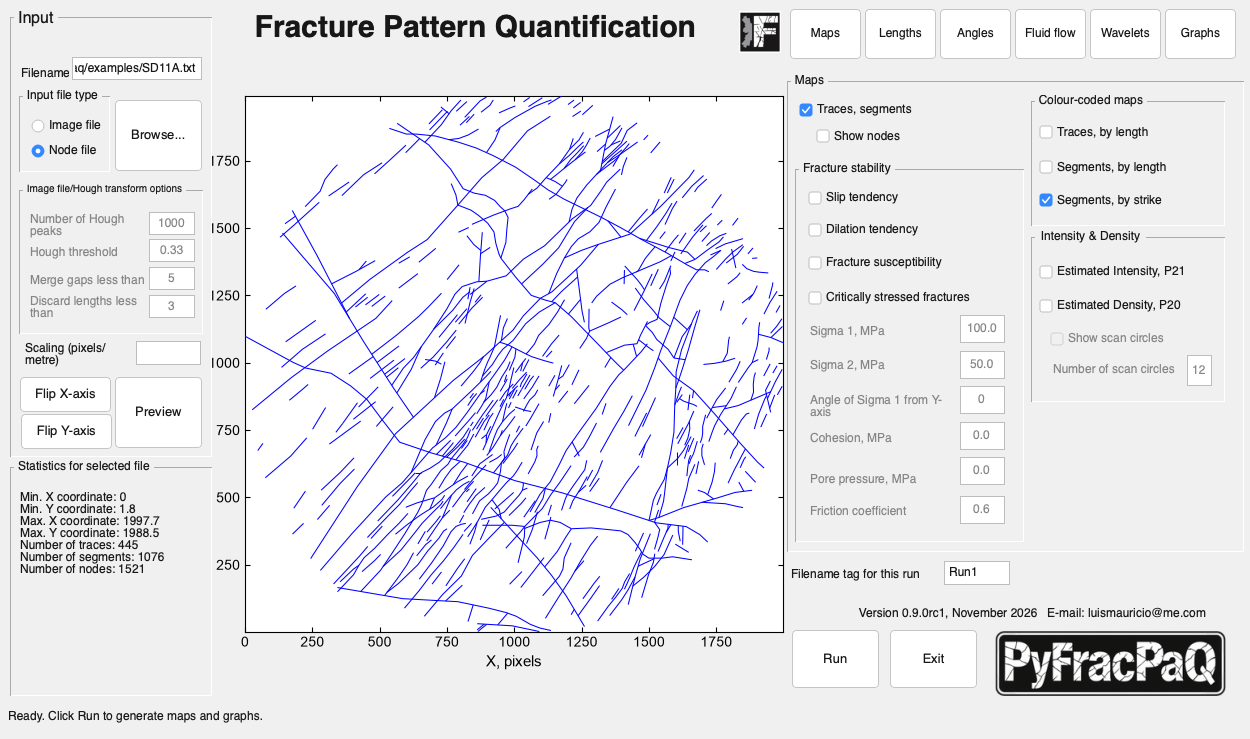
\includegraphics[width=\linewidth]{ui-preview.png}\caption{Actual SD11A preview and statistics. The capture retains the default Run1 tag; use SD11A in the walkthrough to distinguish output files.}\label{fig:preview}\end{figure}

\Needspace{14\baselineskip}
\subsection{Parameters used in this manual's figures}\label{sec:parametros}
The analytical illustrations reuse a reviewed SD11A run with the following parameters, which \emph{are not all GUI defaults}:
\begin{longtable}{@{}p{.43\linewidth}p{.49\linewidth}@{}}
\toprule Group & Illustrated configuration\\\midrule\endhead
Input & No physical scaling or flips; north \(0^\circ\); tag SD11A.\\
Lengths & 20 requested intervals; censoring off; MLE Lower=0 and Upper=0.\\
Angles & 20 requested histogram intervals; \(10^\circ\) rose bins, no length weighting; colour and mean enabled.\\
Maps circular & 12 circles along the shorter side; Show scan circles enabled.\\
Connectivity & 12 blocks; I\(\to\)Y tolerance 2.0 pixels.\\
Stresses & \(\sigma_1=100\), \(\sigma_2=50\) MPa; azimuth \(0^\circ\); cohesion=0, pore pressure=0, friction=0.6. Illustrative values.\\
Permeability & Fixed aperture 0.001 pixel, \(\lambda=1\); no physical calibration.\\
Wavelets & Morlet, a=32, L=2, increment \(90^\circ\). A short demonstration grid.\\
Graphs & Horizontal line from \((0,995.15)\) to \((1997.7,995.15)\); 12 circles.\\\bottomrule
\end{longtable}
Graphs receives points through clicks, rather than coordinate-entry fields. The exact illustrated line was set in the comparison script. An approximate manual selection can change intersections. MLE uses a seed recorded for the illustrated run; the GUI generates its own seeds, so Monte Carlo assessments may vary.

\subsection{States, progress and checking outputs}
Editing the input, scaling, type or Hough parameters invalidates the preview. Run remains disabled until valid geometry is available and while an operation is running. Only parameters needed by the selected analyses are validated. Errors identify the relevant field/tab; choices in other tabs are retained.

Calculations run in the background and figures are presented/exported sequentially through the interface. Wait for completion: MLE and Wavelets can be slow. The main window has no general Cancel button; Exit requests closure at a safe stage. Figures are independent windows with the Matplotlib navigation toolbar. Closing them does not alter the data.
